\documentclass[bibliography=totocnumbered, twocolumn]{article}
\usepackage[left=2cm, right=2cm, top=2cm]{geometry}
\usepackage[tablegrid]{vhistory}
\usepackage{mathptmx}
\usepackage{placeins}
\usepackage{amsmath,amsfonts,bm}
\usepackage[english]{babel} 
\usepackage{listings}
\usepackage{natbib}
\usepackage{graphicx}
\usepackage{rotating}

\usepackage{standalone}
\usepackage{tikz}

\title{EPIC Implementation on the LWA}
\author{James Kent, Jayce Dowell, Adam Beardsley, Nithyanandan Thyagarajan, Greg Taylor, Judd Bowman}

\begin{document}
\maketitle
\begin{abstract}

  Future radio interferometers face a variety of technical challenges related
  to future science goals. These include high performance transient back-ends
  for the detection of pulsars and Fast Radio Bursts (FRB's). Proposed
  interferometers include the SKA-Low which uses a very large number of dipole
  antennas arranged in a very high density layout, which begins to make FX
  correlators practically unfeasible due to them scaling as $\mathcal{O}(n^2)$.
  Thus in future instruments, the computational challenges necessitate a
  paradigm shift in correlator design.

  The MOFF formalism aims to overcome this problem, by re-arranging the canonical
  van-Cittert Zernike theorem to remove the explicit outer product of the vector of
  antenna electric fields, $E(a)$ with its transpose \cite{morales_enabling_2011}.
  This implicit correlation through direct imaging factilitates a scaling of
  $\mathcal{O}(n\log{n})$, providing a significant theoretical advantage for
  future highly dense arrays.

  EPIC is the first practical implementation of the direct imaging correlator
  concept based on the MOFF formalism \cite{thyagarajan_generic_2017}. In this
  paper we describe the practical implementation of a EPIC on the LWA telescope
  in New Mexico, USA, examining the practical details as well as exciting first
  science results.

  
\end{abstract}
\section{Introduction}

Radio astronomy has been undergoing a renaissance in recent years,
with a plethora of new instruments, both built and in the proposal
and design phase. Future  instruments such as the Square Kilometre
Array(SKA) are looking at using high density interferometric arrays
with thousands of individual antennas to facilitate wide field,
high resolution imaging of the sky.

There has also been a renewed focus on observation of transient
phenomena such as pulsar bursts and Fast Radio Bursts(FRB), where
detection and subsequent follow-up imaging data provide significant
technical challenges.

Together, these present a significant computational challenge for
future interferometers, especially with regards to the correlator.
The standard FX correlator, where the signal from one antenna is
multiplied with the signals from every other antenna, which is
mathematically an outer product, scales as $\mathcal{O}(n^2)$,
which becomes problematic as proposed arrays begin numbering in
the thousands of dipole elements.

EPIC represents a significant improvement on this, by scaling as
$\mathcal{O}(n\log{n})$, yielding a significant scaling advantage
for future high density arrays. It also allows imaging the entire
sky in real-time at a high time resolution, down to the microsecond
level, facilitating dragnet surveys of radio transients.

Here, the development of EPIC using the Bifrost framework is
described, and its implementation on the Long Wavelength Array(LWA)
site at Sevilletta in New Mexico, USA. Tenatative science results
are shown, demonstrating its capability for transient detection.

The theory of the MOFF formalism underlying EPIC is described in 
Section \ref{sec:theory}, and a technical description of the
EPIC implementation and development is discussed in Section
\ref{sec:implementation}. First light observations and an initial
meteor transient detection are shown in Section \ref{sec:firstlight},
with benchmarks characterising the performance on the LWA-SV discussed
in Section \ref{sec:benchmarks}, along with an overall discussion in
Section \ref{sec:discussion}.

\section{Theory} \label{sec:theory}

The canonical interferometry formulation is based on the van-Cittert
zernike theorem, from which can be derived the canonical Sky
visibility relationship
\cite{born_principles_1999}\cite{ryle_synthesis_1960}:

\begin{multline} \label{eq:vc}
 I(l,m) = \iint V(u,v,w) \\ \exp\bigg[2\pi i \big(ul + vm + w\big(\sqrt{1-l^2-m^2}-1\big)\bigg]dl\: dm
\end{multline}

Where $V(u,v)$ represents the outer product of all electric fields
with their conjugates:

\begin{align} \label{eq:vis}
  V(u,v,w) = E(u,v,w) \otimes E(u,v,w)^{\ast}
\end{align}

\subsection{MOFF}

The theory of MOFF allows us to re-arrange equation \ref{eq:vc}
to form the MOFF algorithm using the multiplication-convolution
theorem.\cite{morales_enabling_2011}:

\begin{multline} \label{eq:vc}
 I(l,m) = \Bigg\langle \bigg[\iint E(u,v,w) \\ \exp\big[2\pi i \big(ul + vm + w\big(\sqrt{1-l^2-m^2}-1\big)\big]dl\: dm \bigg]^2 \Bigg \rangle
\end{multline}

As per the original MOFF formalism, this can also be expressed
in terms of linear operators, and defining three basis vectors
which the operators transform between:

\begin{align} \label{eq:linformalism}
  I(i) = \Bigg \langle \bigg[ F^T(i,s)M(s,a)E(a)\bigg]^2 \Bigg \rangle
\end{align}

Where $a$ represents the antenna space, $s$ the gridded electric
field space, and $i$ the image space. In this formalism:

\begin{itemize}
  \item $E(a)$ - Represents a vector of fourier electric field values.
  \item $M(s,a)$ - Represents the mapping of the individual electric field values to the fourier grid, convolved with the antenna illumination pattern and other convolutions such as wide field effects.
  \item $F^T(i,s)$ - Inverse fourier transform to image space.
\end{itemize}

This defines gridding an electric field pattern directly for each
antenna followed by a fourier transform to produce the image. This is
followed by squaring the image, or cross multiplying between
polarisations, and accumulating images over time.

This produces what are commonly called `dirty images', which is the
true sky brightness distribution convolved with the point spread
function of the instrument.

\subsection{Implications}

The MOFF algorithm is the cornerstone of EPIC and scales as
$\mathcal{O}(n\log{n})$, compared to $\mathcal{O}(n^2)$ for the
classical FX correlator. This is a great improvement in the
context of future, highly dense arrays, where, depending on
array geometry, an FX correlator may be less efficient than
an EPIC based correlator \cite{thyagarajan_generic_2017}.
The limiting factor for MOFF is the FFT size from the grid,
whereas an FX correlator is the number of baseline pairs.

An additional characteristic of the MOFF formulation is the
lower data rates implicit in outputting small FFT images at
high time cadence compared to visibilities. This means that
the sky can be imaged at a higher time resolution than is
possible using an FX correlator. The ramifications for EPIC,
as will be seen, is that all-sky imaging at millisecond-level
sampling periods can yield new insight into radio transient
phenomena.

\section{Implementation} \label{sec:implementation}

The EPIC pipeline has been implemented on the Long Wavelength Array (LWA)
site at Seviletta in New Mexico. First light was achieved in late
August 2018 with no modifications to the correlator software apart
from swapping the standard FX correlator for the MOFF based correlator: EPIC.


\subsection{Long Wavelength Array}

The LWA is an interferometer observing
between frequencies of 20MHz to 120MHz, with two operational stations
located at the VLA Site and Seviletta, both in New Mexico, USA \cite{henning_first_2010}\cite{taylor_first_2012}. Its
high density configuration makes it an excellent candidate for
deployment of EPIC .

It consists of 256 dipole antennas arranged in a dense pseudo-random
arrangement on a fairly flat piece of ground. One of the antennas
sits further from the array, acting as an outrigger to improve the
angular resolution of the telescope. This outrigger was explicitly
excluded during our implementation to ensure a high density, keeping
the resultant FFT size as small as possible.

Each dipole signal is initially digitized on the antenna, and transmitted via
fibre-optic cable back to the central correlator, where a hardware
front-end performs initial bandpass filtering and applies
appropriate gains. The signals are than routed into a bank of
Xilinx FPGA's which perform an accumulation and fourier transform
for each channel, producing a fourier sample every 40uS.

These samples are routed over a high performance local ethernet
connection to a rack comprising sixteen general purpose computer
clusters, equipped with Intel Xeon processors and two NVIDIA GTX 980's
each.

EPIC was deployed initially on a single node, processing a part of
the LWA's bandwidth. We will later examine how much bandwidth can
be processed on EPIC versus a standard FX correlator, and the parameters
affecting it.

Deployment on the LWA has been supported and sped up greatly through
the LWA's extensive public software library which trivialises steps such as
performing delay calibration to account for different antenna lengths,
as well as storing the array geometry \cite{dowell_long_2012}.

\subsection{Bifrost}

The implementation is done using the Bifrost framework
\cite{cranmer_bifrost:_2017}. Bifrost is a highly abstracted library
for building high performance streaming systems. The back-end
framework is built using C++ which calls high speed CUDA libraries
and bespoke kernels implemented by the Bifrost Developers. For
ease of use an abstracted python front-end is provided.

Bifrost is based around the concept of blocks, where each block performs
some operation on the data, and then outputs it into a high-speed
ring buffer in memory, which facilitates moving data between blocks.
The output ring buffer from one block becomes the input ring buffer
for the next block. Each block removes a block of data, termed a
'gulp' from the ring, processes it before placing a gulp into
the output ring. The block processes data until the input ring is emptied
or the pipeline is shutdown.

Many standard signal processing techniques are implemented into
the bifrost back-end with GPU capability where appropriate. These
include operations such as FIR Filters, Fast Fourier Transforms,
and various matrix algebra operations.

The python front end also includes a high performance mapping
function which takes a string of C++/CUDA and uses a Just-In-Time (JIT)
compiler to generate and execute valid CUDA code on-the-fly. The
power of this feature cannot be understated, and is responsible
for a lot of EPIC's success.

The majority of the EPIC implementation in Bifrost was done using the
standard signal processing blocks as well as the bifrost map function,
with a notable exception of high-speed convolution and gridding, for
which a custom kernel was created based on a high speed gridder
developed by John Romein in the Netherlands
\cite{romein_efficient_2012}.

\subsection{Pipeline}

The real-time streaming processor implementation constitutes an
several Bifrost blocs. An overview of each of these blocks is shown
in Figure \ref{fig:pipeline}.

The design of the LWA correlator includes filtering and digitizers in
a high speed hardware front-end, with additional accmulation and
fourier transform and binning done on FPGA's, which output an
amplitude value for each channel every 40us. This data is broadcast
via UDP over a high speed local ethernet connection to a set of
general purpose compute clusters equipped with standard CPU's and two
high speed NVIDIA GPU's each.  The GPU's in use for this
implementation are NVIDIA GTX 980's.

The cluster element is everything after the first block in Figure \ref{fig:pipeline}.
It constitutes a python program running Bifrost, with all significant
compute and memory operations done seamlessly through access to the
high performance C++/CUDA backend.

The data from the FPGA's is received via UDP in a 4+4-bit complex
format.  This services to reduce the bandwidth requires by the local
ethernet connection.  The channelised fourier data is first transposed
to move the data ordering from $\big[Time, Channel, Antenna,
Polarisation\big]$, to $\big[Time, Channel, Polarisation,
Antenna\big]$. This is important as it facilitates contiguous loads in
the romein step, discussed below.

After the transposition operation, the 4+4-bit complex number is
unpacked to to a standard 64-bit complex number (32-bit real, 32-bit complex)
and delay calibration for antenna cables is applied using a high
speed Bifrost map function. The delay calibrated data is then
convolved with the antenna illumination pattern, which is a user-defined
convolution kernel. For the LWA a simple square top-hat function was
used. This is then gridded onto a 2D grid with a spacing of $\frac{\lambda}{2}$
to ensure we are not sampling fourier modes outside of a physical horizon.

This convolution and gridding operation is done using the Romein
convolution algorithm, designed specifically for high speed
visibility gridding where locality is poor and memory bandwidth
is high \cite{romein_efficient_2012}.

Once the data has been gridded for a simple 40uS time step, the
grid is inverse fourier transformed to produce an image of the
sky. These images are then accumulated to a user-defined time
depending on the science use case. Once an image has accumulated
to the threshold time, it is dumped to disk and converted to a FITS
image in a post-processing step. This ensures the streaming service
isn't held up by high-cost image manipulation operations.

Optionally autocorrelation removal can also be done to remove
the zero-spacing power inherent in the MOFF algorithm. The
imprint in the image of the gridding illumination kernels, can be removed
after the fact in a post-processing step as they are
pre-generated and thus known previously.


\begin{figure}
  \centering
  \scalebox{0.5}{\includestandalone{images/pipeline}}
  \caption{EPIC Implementation block diagram. Each block represents a Bifrost block, and each arrow a high speed ring buffer for moving data fast and in real time.}
  \label{fig:pipeline}
\end{figure}

\subsection{Romein}

The Romein convolutional algorithm proved to be a critical
step in the implementation of EPIC. Previous EPIC reference codes
have attempted to use a direct convolution mapping using a matrix,
as described by the operator formalism in \cite{thyagarajan_generic_2017}.

Unfortunately on a GPU this results in unacceptably high
memory bandwidth which serves to cause this step to bottleneck
the code significantly. The Romein convolution was used instead as it
is designed to reduce the GPU memory bandwidth significantly
by only doing explicit memory store operations when necessary.
The algorithm is designed to preferentially accumulate any grid
updates a in high speed local register on the GPU core.

Romein additionally allows multiple convolution kernels to be
combined together and applied simultaenously. This not
only allows convolution of the fourier point with the
illumination pattern, but additionally scope for wide-field
and antenna effects, such as is implemented in W-Projection \cite{cornwell_noncoplanar_2008}.

The implementation of non-coplanarity correction to ensure
wide field fidelity will be covered in a future paper looking
at EPIC for wide-field effects.

The Romein convolution was implemented by modifying the Bifrost
back-end and adding the necessary kernels, written in C++/CUDA. The
additional Bifrost module is intended to be a generic, type-agnostic
convolution kernel. This is then called through the ctypes interface
from the main EPIC script.

\section{First Light} \label{sec:firstlight}

The initial deployment of EPIC took place on the LWA-SV site
during the week of the 27th-31st August 2018.

The first few hours of observations were ran at an image of
accmumulation time of 25 ms, to allow observation of any
transient phenomena in the radio sky at that time. The bandwidth
used was approximately 800 khZ running with dual polarisations. 

\subsection{Meteor Transients}

During the initial run of observations, the system was left to
run at a high time cadence of 25 ms, imaging the whole sky. This
allowed us to see wether the LWA could detect any strong radio
transients and image them in real-time.

Over several hours, multiple small transients were noticed. The
majority of them are RFI, which most often shows up on the horizon
or as a large all-sky distortion. The RFI environment at the LWA
Seviletta site is fairly good, however there are nearby in-band
transmitters. There is also line of sight between the array and
the nearby I-25 interstate, thus there is some interference from
passing traffic.

After ruling out RFI effects, some transients were noticed, the
brightest of which in our observing window was a meteor striking
the earths atmosphere, a still frame of which is shown in Figure~\ref{fig:meteor}.
The meteor striking the atmosphere generates a plasma, which acts
as a reflector for an over the horizon TV transmitter, which
serves to illuminate meteors plasma path.

Using this approach, and operating EPIC continously, we hope to
detect other similar meteor events in addition to other
transient phenomena where EPIC has a unique capability due to
its all-sky imaging at high time resolution. This effectively
allows it to act as an all-sky imaging dragnet for transient radio
events. 


\begin{figure}
  \centering
  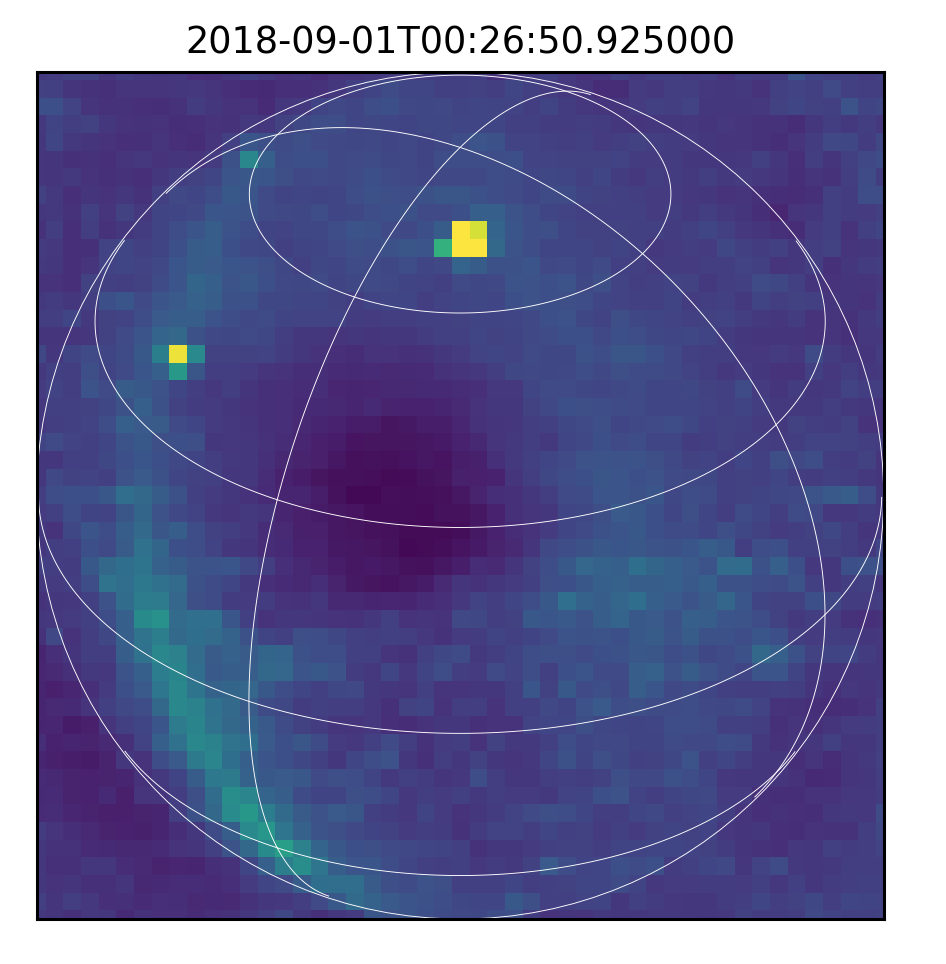
\includegraphics[width=0.4\textwidth]{images/meteor.png}
  \caption{Meteor Detection during an observation on the LWA-SV site. The plasma left by the meteor impacting the atmosphere reflects off an over-the-horizon 55 MHz TV transmited, and this is what we are observing here.}
  \label{fig:meteor}
\end{figure}


\section{Benchmarks} \label{sec:benchmarks}

During the first light deployment at the LWA-SV site, the
performance was measured and characterised. The performance
is both a consequence of both the deployment system and
hardware, as well as EPIC's execution method in comparison
to an FX correlator.

Overall, in the first iteration, 800 kHz of bandwidth is available
per GPU card on the LWA-SV correlator, when running with only
a single polarisation, which is useful for maximising bandwidth
for faint transients facilitating averaging over the band. With
the LWA-SV system's current hardware layout, this facilitates
12.8 MHz of single polarisation bandwidth.

When running with both X and Y polarisations, which allows the
formation of pseudo-stokes images for more precision radio
surveys, half the overall bandwidth is available: 400 kHz
per card, and 6.4MHz for the entire system if all nodes are
running EPIC.

\subsection{Maximum Throughput}

To characterise the overall throughput of the system, we monitored
the UDP streams being broadcasted by the FPGA cards running the
front-end fourier transforms and frequency binning. If the
system was keeping up reasonably well, then packet loss would be
almost nothing. If compute requirements increased on the node,
by increasing the number of channels per card, or the frequency
tuning, necessitating a larger FFT size, then you will notice
packet loss as the pipeline struggles to keep up with the
incoming data stream.

The best rule of thumb we have discovered is to look at the time
'gulp', i.e the amount of time represented by a single chunk of
data, and ensure that the system can process that in a slightly
shorter amount of time. For example, if ingesting 50 ms worth
of data in a single gulp from the ring buffer, to ensure the
system can keep up, the GPU should process it in at least 45ms
or so. There are additional overheads in the system, such as
running a normal Linux operating system in the back-ground,
so system processes might cause the occassional hiccup in
processing.

The results of our initial tests on the system are shown in
Figures \ref{fig:singlepol_time} and \ref{fig:doublepol_time}. The
system shows good stability when running at a reasonable setting
and tuning.

\subsection{GPU Performance}

An additional point of interest is the overall performance and
suitability of EPIC on a GPU programming model, and characterising
that.

An FX correlator is fairly simple in that it performs an outer
product of the vector of electric fields with the transpose of
itself. This is also an absolutely superb fit for the GPU
programming model, as it is almost completely compute bound. This
is best explored using a roofline model, a common visualisation in
high performance computing to analyze the execution properties
of a particular algorithm \cite{demmel_roofline:_2008}.

The roofline comparison between for the GPU computed elements of an
FX correlator and EPIC is shown in Figure \ref{fig:epic_roofline}.
As can be seen the FX correlator is exceptional in that it is
compute bound, whereas EPIC is very much memory bound. This means
increasing total amount of compute power would not be as beneficial
to EPIC, compared to increasing the memory bandwidth available to it.

This is one of the reasons why an FX correlator is able to process
more bandwidth than an EPIC based correlaton. Also EPIC is a
full-scale imager running in real-time, as the correlation
operation that is explicit in an FX system is implicit in the
EPIC imaging. 

\begin{figure}
  \centering
  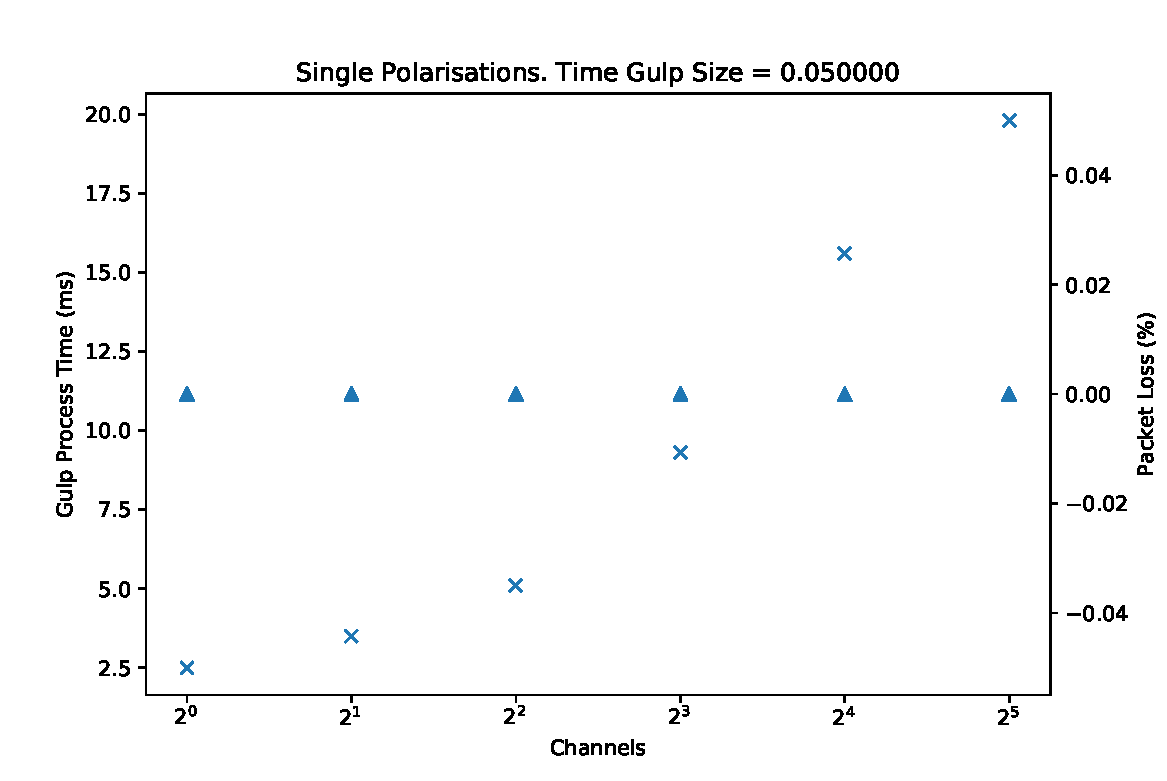
\includegraphics[width=0.5\textwidth]{images/single_pol_throughput.pdf}
  \caption{Processing time per 'gulp' as a function of the number of channels being processed, for only XX polarisation.}
  \label{fig:singlepol_time}
\end{figure}

\begin{figure}
  \centering
  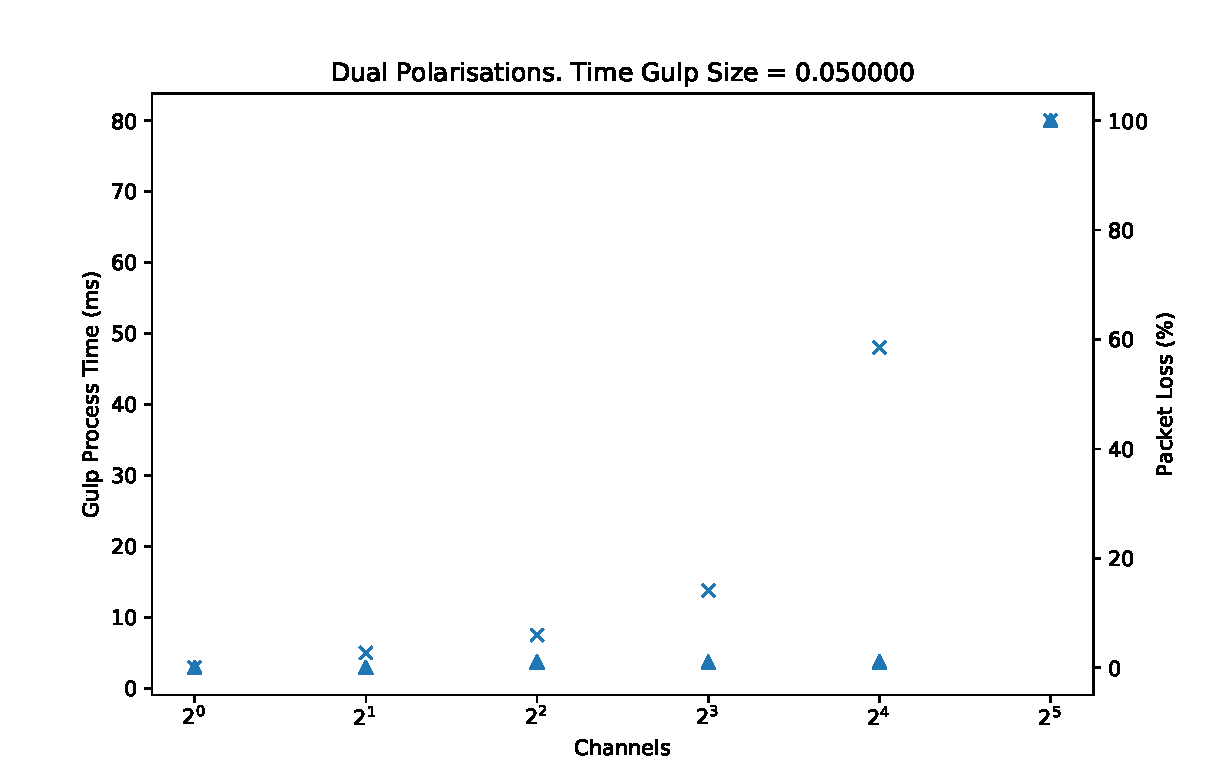
\includegraphics[width=0.5\textwidth]{images/dual_pol_throughput.pdf}
  \caption{Processing time per 'gulp' as a function of the number of channels being processed for XX, XY, YX and YY cross-polarisations.}
  \label{fig:doublepol_time}
\end{figure}

\begin{figure}
  \centering
  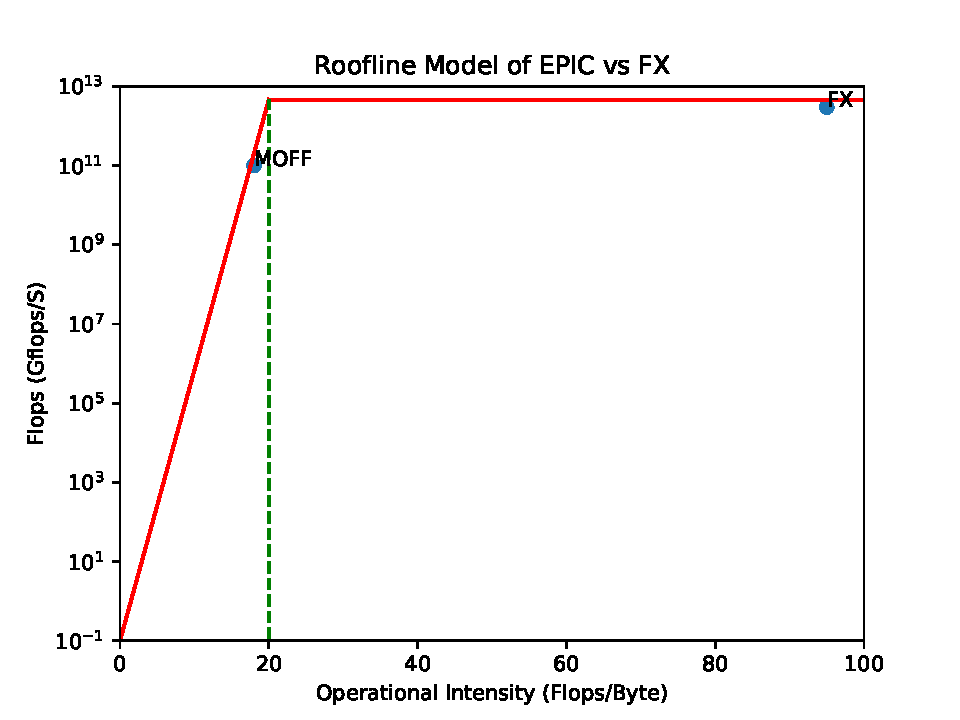
\includegraphics[width=0.5\textwidth]{images/epic_fx_roofline.pdf}
  \caption{A roofline model comparing an FX correlator outer product with the EPIC pipeline.}
  \label{fig:epic_roofline}
\end{figure}


\section{Discussion} \label{sec:discussion}

The development, and commissioning of EPIC has yielded a functioning
direct imaging correlator. The tentative observations of transient
phenomena is greatly encouraging for future science cases. EPIC's all
sky imaging capability with high time resolution, opens a window into
interesting radio transient phenomena due to its imaging capacity.

The development and commissioning of EPIC took place over a period of
eight weeks. The reason for this exceptionally quick turnaround was
power of the Bifrost framework underlying the correlator. It painlessly
implements the infrastructure required to build a high throughput
streaming and data processing system.

The C++/CUDA back-end abstracts away complicated and precise constructs
such as the ring buffers, which form the communication backbone between
processing steps. The major advantage is the native CUDA support,
trivialising accessing the power of the GPGPU paradigm. Extending the 
Bifrost framework, such as adding extra GPU-enabled processing blocks, as
was done during development, is straightforward due to the flexible
architecture.

Future work will be focused around several elements:

\begin{itemize}
\item EPICal - EPIC requires calibration in real-time. A solution has been demonstrated but not implemented in a working correlator \cite{beardsley_efficient_2017}. This will be the a major feature addition.
\item Wide Field Effects - It is necessary to deal with non-coplanarity and wide fields effects in EPIC. A forthcoming paper will elucidate the principles and practicalities behind doing this on direct imaging correlators.
\item Optimisation - EPIC has unique computational challenges associated with it, which will benefit from broad and aggressive optimisation of key kernels and bottlenecks such as the convolutional gridding and FFT's.
\end{itemize}

Implementing EPICal is of particular importance for providing scientific
observations of the sky in an astronomical unit such as Kelvin's
or Jansky's. Currently images are not calibrated, therefore, information
is only available through the relative scale of the images.

Future technical improvements include a correction of wide field
effects, similar to what is done with visibilities using W-Projection \cite{cornwell_noncoplanar_2008}.
Additionally EPIC needs to be optimised to run on a wide variety of generic
GPU-enabled clusters to facilitate expanding its instrument base further.

\section{Conclusion}

The first version of a working EPIC correlator has been developed
fully, and its implementation and operation demonstrated at the
LWA-SV site. Some exciting first observations of meteor transients
have been made, and future papers will examine the scientific
output of EPIC in more detail.

EPIC is an example of a high throughput CUDA-enabled streaming system
built on the Bifrost framework, facilitating rapid development of what
was previously an exceptionally laborious task. Future optimisation
will centre around using the flexibility it offers in creating custom
hand-optimised CUDA kernels to ensure efficient on execution on a
wide variety of hardware, enabling deployment on a diverse set of
correlator infrastructure.

Future work will involve the implementation of the real-time
calibration pipeline, and correcting for wide field distortion
effects. The exceptional progress on the initial deployment of
EPIC is greatly encouraging for future scientific results.


\bibliographystyle{apalike}
\bibliography{references_all}{}

\end{document}